
\section{Results}

\subsection{Simulation Results}

We begin by illustrating the performance of the \textit{CorShrink} method on simulated data. We randomly generated covariance matrices of dimensions $p$ varying in the range $100$, $500$ and $1000$ and then generated $n$ samples from a Multivariate Normal distribution centered at $0$ and with the above generated covariance matrix. We considered four choices of $n = 5, 10, 50, 200$ that spans all three scenarios -  $n << p$, $n <p$ and $ n > p$.  We then performed shrinkage on the sample covariance matrix using the three versions of \textit{CorShrink}, GLASSO at 4 different regularization parameter values ranging from low to high shrinkage and the Sch\"{a}fer-Strimmer method \cite{Friedman2008} \cite{Witten2010} \cite{Schafer2005}. 

In Figure \ref{fig:fig1}, we compare the eigenvalues of the shrunk covariance matrices under different shrinkage schemes and different choices of $n$ for $p=100$. Results corresponding to other choices of $p$ can be checked here [?Link].    Figure \ref{fig:fig1} shows that the trends of the eigenvalues from the \textit{CorShrink-ML},  \textit{CorShrink-VEM2} and Sch\"{a}fer-Strimmer shrinkage methods are consistently close to the population eigenvalues across all four choices of $n$. The \textit{CorShrink-VEM} version performs well for the $n <<p$ scenarios, however its performance is not so good for moderate to large values of $n$. This is probably due to the fact that for larger data, the strong weight of the Dirichlet hyperprior on the null component and the fixed grid of component variances of underlying mixture model on Fisher Z-scores makes the model inflexible to adapt itself to data, a problem that is solved in VEM2 when the component variances are more flexibly chosen by the model. GLASSO for low shrinkage ( regularization parameter $\rho = 0.05$) is very close to the sample covariance matrix and for high shrinkage ($\rho=10$) provides a matrix close to diagonal and therefore is a bad fit to the population covariance matrix. The $\rho=0.5$ or $\rho = 1$ provide slightly better fit to the population covariance matrix in terms of eigenvalue patterns, but noticeably, for $n << p$ cases, the top eigenvalues (with the highest magnitude) remain very close to that of the sample covariance matrix despite increasing the level of shrinkage and it is the lower order eigenvalues that adapt more rapidly with increasing $\rho$. Here we must emphasize that usually, the top few eigenvalues are of principal interest to researchers interested in lower dimensional representation, and under $n << p$ scenario, the three versions of the \textit{CorShrink} approach and the Sch\"{a}fer-Strimmer shrinkage method are more effective than GLASSO in mapping the top eigenvalues close to the ones from the population covariance matrix. 

%The sample covariance matrix  for $n <<p$ has few non-zero eigenvalues since its rank is $\leq n$, and therefore, fits the population eigenvalue structure badly. 
\begin{figure*}[ht]
\raggedleft
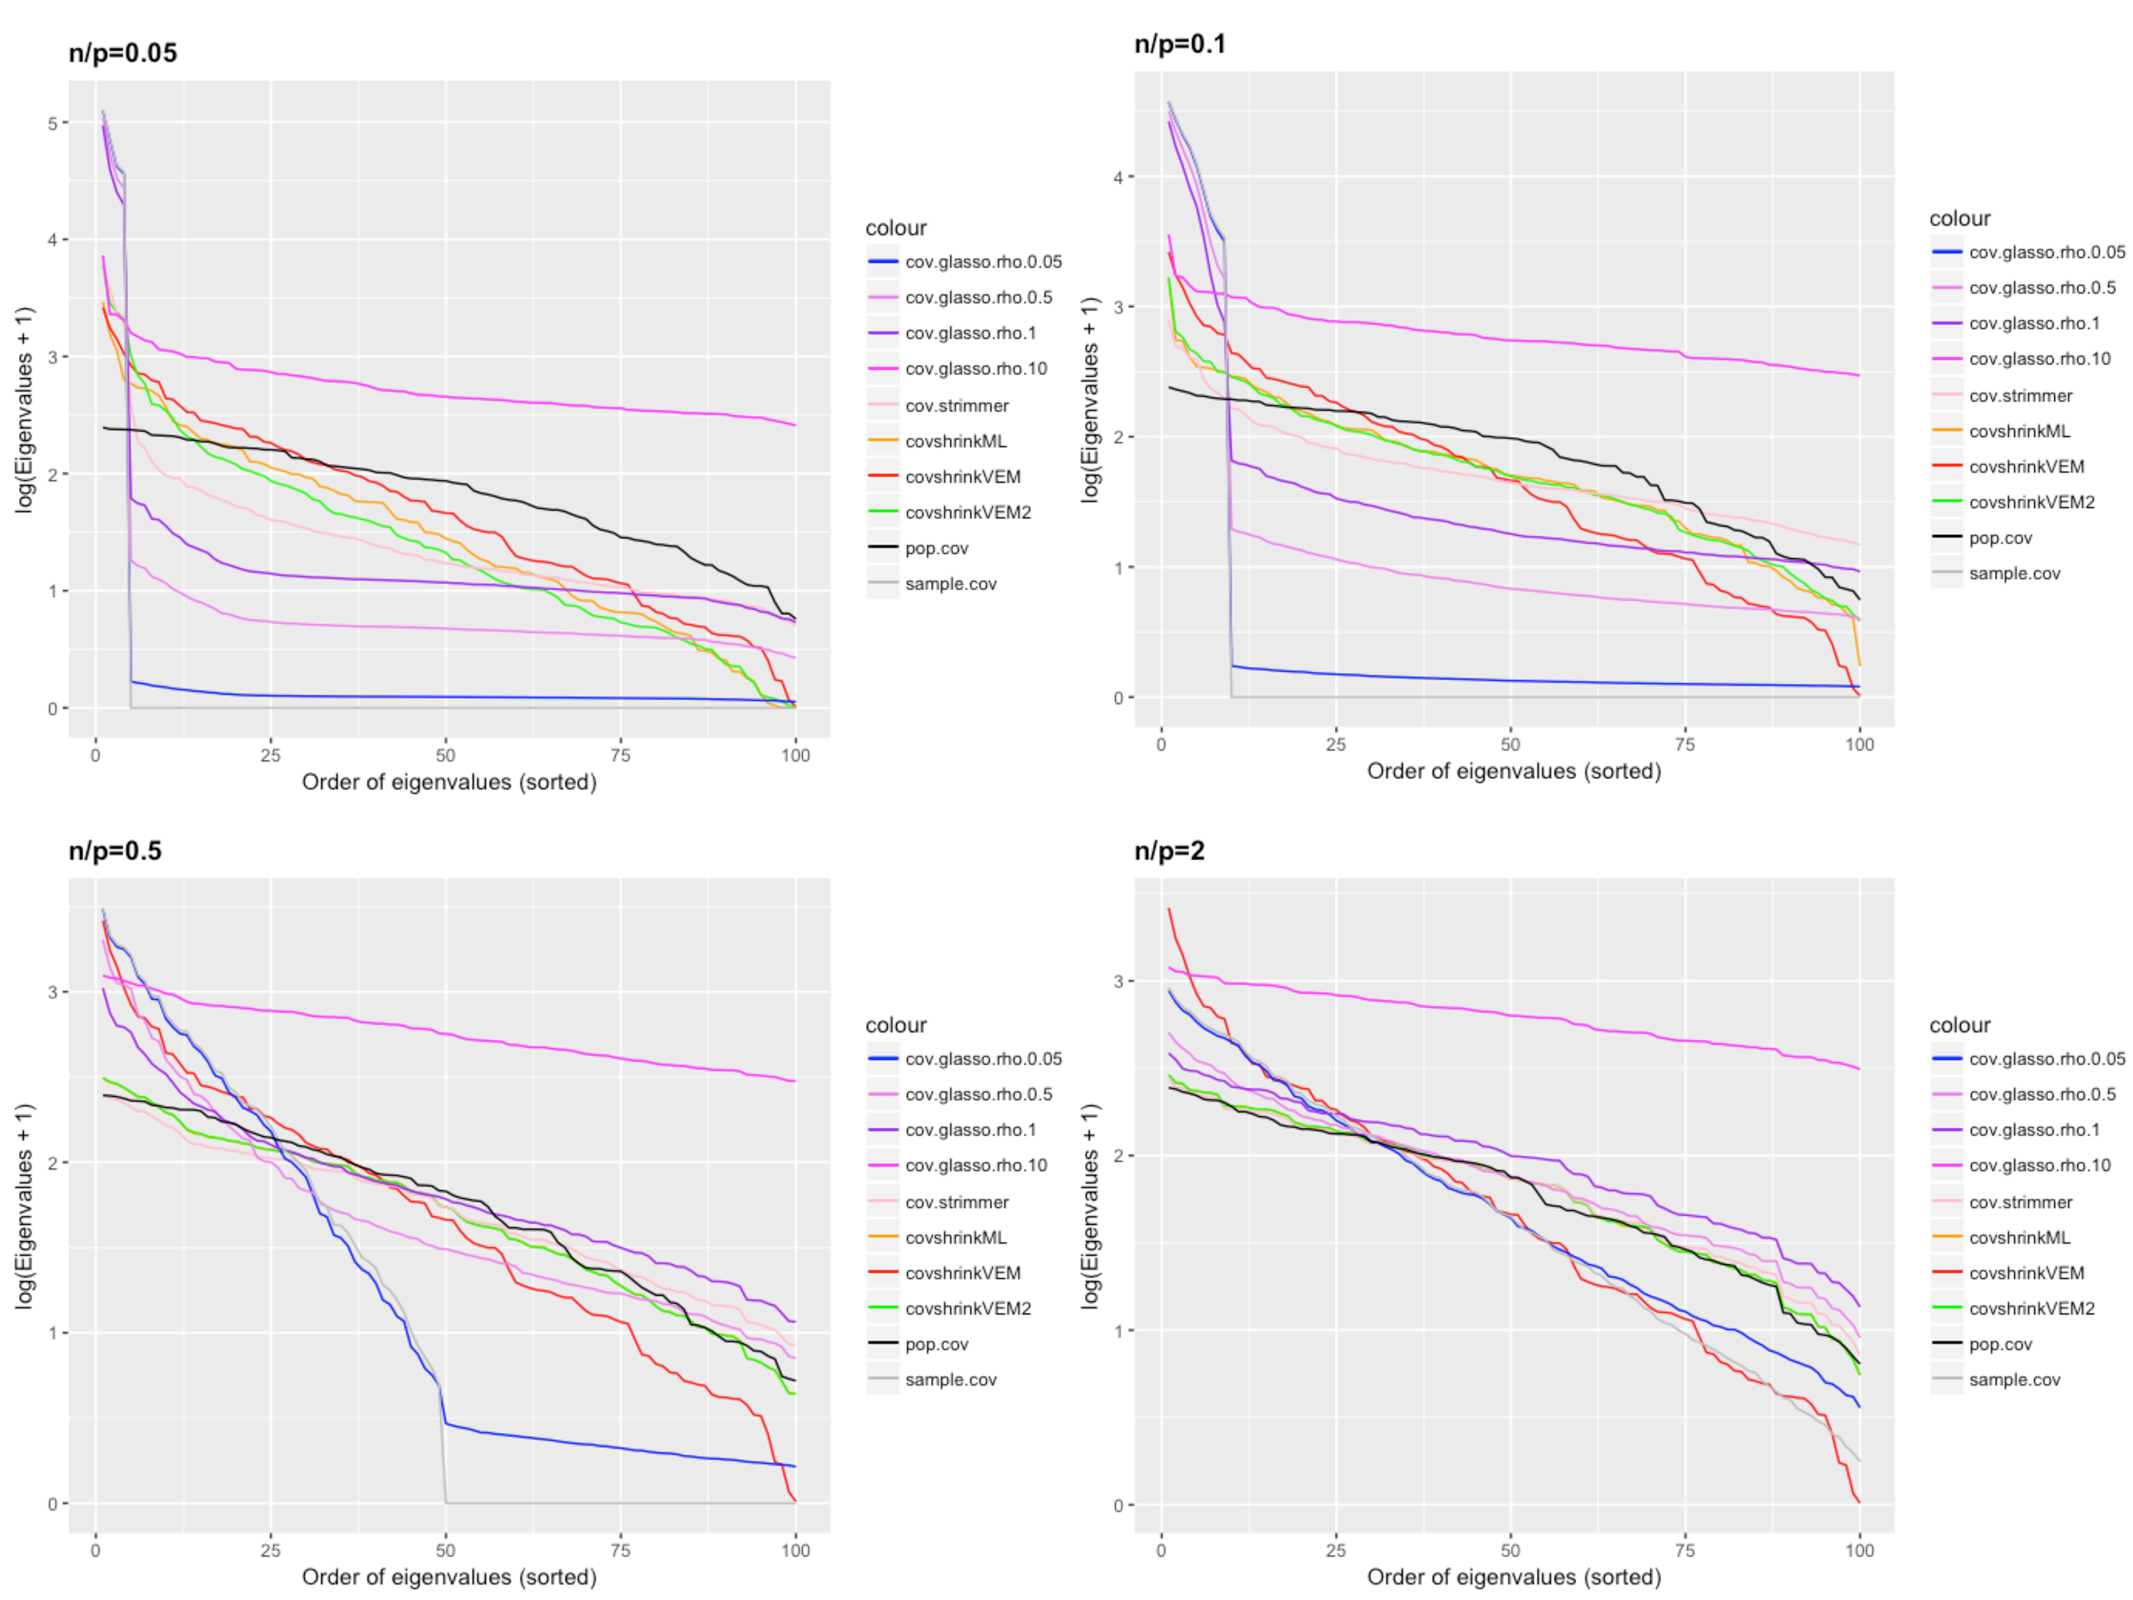
\includegraphics[height=3in, width=6in]{eigenval_dist_2.pdf}
 \caption{Distribution of the sorted eigenvalues for the shrunk covariance matrices due to the three versions of \textit{CorShrink}- namely \textit{CorShrinkML}, \textit{CorShrinkVEM} and \textit{CorShrinkVEM2}, three versions of GLASSO for three regularization parameters $\rho$, varying from $0.05$, $0.5$ and $1$  [ low to high shrinkage ] and the Sch\"{a}fer-Strimmer shrinkage method, along the distributions of the eigenvalues for the sample covariance and the population covariance matrices.}
\label{fig:fig1}
\end{figure*}

Besides the eigenvalue trends and the top few eigenvalues, another important consideration in comparing these shrinkage methods is how close the eigenvectors from the shrunk covariance matrices are with respect to the population covariance matrix. Table ~\ref{tab:tab1} present the average distance between the top 5 eigenvectors of the each shrinkage method with respect to the population covariance. Again we find that the Sch\"{a}fer-Strimmer, \textit{CorShrink-ML} and \textit{CorShrink-VEM2}  produce shrunk covariance matrices closest to the population covariance matrix in terms of the eigen-spaces corresponding to the top eigenvalues. In Figure \ref{fig:fig2}, we plot the distribution of the correlations from the shrunk matrices obtained using different shrinkage methods . We observed that the distribution is more concentrated around $0$ for the  \textit{CorShrink} models when compared to the GLASSO and Sch\"{a}fer-Strimmer methods. Additionally,  \textit{CorShrink} retains some correlation values with large magnitudes. This characteristic of the  \textit{CorShrink} approach would ensure a sparse representation when used in building correlation networks.




\begin{figure*}[ht]
\centering
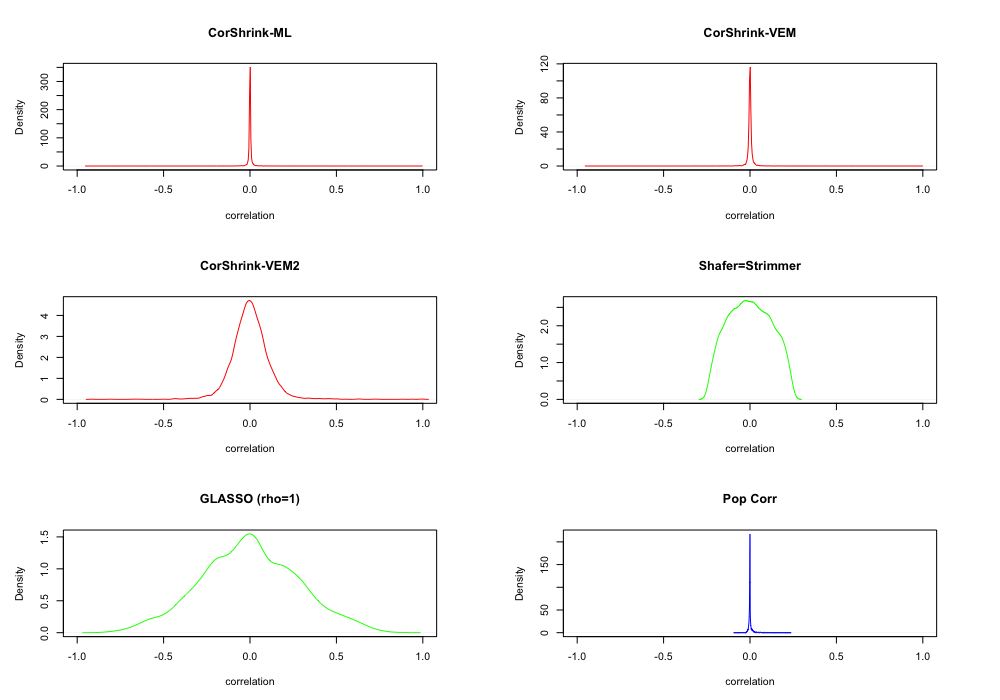
\includegraphics[height=2.5in, width=5in]{correlation_density_compare}
 \caption{Overall distribution of the correlations after shrinking the covariance matrix using the three models of \textit{CorShrink}, Sch\"{a}fer-Strimmer method and the GLASSO method for regularization parameter of $1$ (which was found to be the best fit in terms of eigenvalue patterns out of the four choices considered). The correlation distributions are compared with the actual correlation distribution from the population covariance matrix.}
\label{fig:fig2}
\end{figure*}

\clearpage
\begin{table}[ht]
\begin{center}
\caption{Average Distance of the first 5 eigenvectors of the shrunk covariance matrices from different shrinkage methods versus population covariance matrices. \label{tab:tab2}}
\begin{tabular}{|p{1.5in}|p{0.8in}|p{0.8in}|p{0.8in}|p{0.8in}|}
 \hline
 Methods &  $n/p=0.05$ & $n/p=0.1$ & $n/p=0.5$ & $n/p=2$ \\ \hline
 CorShrink-ML & 0.030 &  0.034  &  0.033  &  0.036 \\ \hline
 CorShrink-VEM  &  0.037  &  0.039  & 0.057  & 0.062 \\ \hline
 CorShrink-VEM2 & 0.031 & 0.046 & 0.043 & 0.037 \\ \hline
 Sch\"{a}fer-Strimmer & 0.037 & 0.054 & 0.051 &  0.044 \\ \hline
 GLASSO ($\rho=0.05$) & 0.083 & 0.085 & 0.085 & 0.069 \\ \hline
 GLASSO ($\rho=0.1$) & 0.078 & 0.083 & 0.084 & 0.061 \\ \hline
 GLASSO ($\rho=0.5$) & 0.064 & 0.081 & 0.081 & 0.057 \\ \hline
 GLASSO ($\rho=1$) & 0.063 & 0.079 & 0.080 & 0.057 \\ \hline
 Sample cov  & 0.083 & 0.084 & 0.085 & 0.076 \\ 
 \hline	
\end{tabular}
\end{center}
 \end{table}
 
 \section{Discussion}
 
Our goal here is to highlight the potential of the \textit{CorShrink} models in performing adaptive correlation and covariance shrinkage that has comparable to better performance over the Sch\"{a}fer Strimmer shrinkage approach in terms of eigen-space and eigenvalue patterns comparisons and that outperforms GLASSO as a correlation shrinkage method irrespective of the choice of regularization parameter used for the latter (see Figure~\ref{fig:fig1} and Table \ref{tab:tab1}).
In terms of computational time, the computation time for the \textit{CorShrink-ML} method is comparable with GLASSO under medium to high shrinkage and Sch\"{a}fer Strimmer method, while \textit{CorShrink-VEM} and \textit{CorShrink-VEM2} are slower in comparison. For instance, the time taken to run \textit{CorShrink-ML}, \textit{CorShrink-VEM} and \textit{CorShrink-VEM2} on the Deng et al samples data were ?? , ??  and ??  seconds whereas that for GLASSO ($\rho =1$) and Sch\"{a}fer-Strimmer methods were ??  . 

The \textit{CorShrink} can be easily extended to partial correlation and partial covariance matrices and also leads to efficient computation of the inverse correlation and covariance matrices. The latter would allow one to build causal networks based on the \textit{CorShrink} models and compare them to the GLASSO based causal networks. An example of a causal network on the samples of the Deng et al data using  the three shrinkage approaches \textit{CorShrink-ML}, Sch\"{a}fer-Strimmer and GLASSO ($\rho=1$) is provided here. This method also opens other areas of applications and extensions that we intend to pursue in future. One can combine Linear Discriminant Analysis and  Multiple regression problem with the shrunk covariance matrices obtained from the \textit{CorShrink} approaches, in the same way the Sch\"{a}fer Strimmer method has been used in these domains \cite{Xu2009} \cite{Schafer2005}. In this paper, we did not consider any additional structure on the covariance matrices. But for structured covariance matrices, one would want to pool the knowledge of the structure into the shrinkage method. For example, for a block covariance matrix, it makes more sense to apply \textit{CorShrink} separately on each block and pool the blocks together. 


The codes to fit the \textit{CorShrink} models on data are implemented in an R package \textbf{CorShrink} which is available on Github at \url{https://github.com/kkdey/CorShrink}. It also contains a README demonstrating how these models could were fitted on simulated data. The Deng et al single cell data \cite{Deng2014} is available as a R data package with instructions for downloading and loading into R at \url{https://github.com/kkdey/singleCellRNASeqMouseDeng2014}.

\begin{thebibliography}{9}

\bibitem{Ledoit2003}
Ledoit O. and Wolf  M. 2003. 
"Improved estimation of the covariance matrix of stock returns with an application to portofolio selection.
\textit{Journal of Empirical Finance}. 10 (5): 603?621.

\bibitem{Ledoit2004}
Ledoit O. and Wolf  M. 2004. 
Honey, I shrunk the sample covariance matrix.
\textit{The Journal of Portfolio Management}. 30 (4): 110?119.

\bibitem{Lancewiki2014}
Lancewicki T. and Aladjem M. 2014.
Multi-Target Shrinkage Estimation for Covariance Matrices.
\textit{IEEE Transactions on Signal Processing}. 62 (24), 6380-6390

\bibitem{Schafer2005}
Sch\"{a}fer J and Strimmer K.  2005. 
A shrinkage approach to large-scale covariance matrix estimation and implications for functional genomics. 
\textit{Statist. Appl. Genet. Mol. Biol}.4.32.

\bibitem{Schafer2005b}
Sch\"{a}fer J and Strimmer K.  2005. 
An empirical Bayes approach to inferring large-scale gene association networks. 
\textit{Bioinformatics}. 21: 754-764.

\bibitem{Stephens2016}
Stephens M. 2016. 
False discovery rates: a new deal. 
\textit{Biostatistics} Advance Access.


\bibitem{Deng2014}
Deng Q,  Ramskold D,  Reinius B,  Sandberg R. 2014.
Single-Cell RNA-Seq Reveals Dynamic, Random Monoallelic Gene Expression in Mammalian Cells.
\textit{Science}.  343 (6167) 193-196.

\bibitem{Xu2009}
Xu P.,  Brock GN,  Parrish RS.  2009.
Modified linear discriminant analysis approaches for classification of high-dimensional microarray data.
\textit{Computational Statistics $\&$ Data Analysis}. 53.5.

\bibitem{Friedman2008}
Friedman J,  Hastie T,  Tibshirani R. 2008.
Sparse inverse covariance estimation with the graphical lasso. 
\textit{Biostatistics}. 9.3.

\bibitem{Witten2010}
Witten DM,  Friedman JH, Simon N. 2010.
New Insights and Faster Computations for the Graphical Lasso. 
\textit{Journal of Computational and Graphical Statistics}, 20, 4, 892?900.

\bibitem{Blei2016}
Blei DM, Kucukelbir A, McAuliffe JD. 2016.
Variational Inference: A Review for Statisticians.
https://arxiv.org/pdf/1601.00670.

\bibitem{Beal2003}
Beal MJ, Ghahramani Z.
The Variational Bayesian EM Algorithm for Incomplete Data: with Application to Scoring Graphical Model Structures
\textit{Bayesian Statistics}, 7.


\end{thebibliography}



